% Built on the official CVPR 2027 author kit (https://github.com/cvpr-org/author-kit).
\documentclass[10pt,twocolumn,letterpaper]{article}

\usepackage[review]{cvpr}
%% This file contains a number of tweaks that are typically applied to the main document.
%% They are not enabled by default, but can be enabled by uncommenting the relevant lines.


%%
%% Official support for 2-column teaser figure
%%
\usepackage{cuted} %< for strip environment

%%
%% For auto-referencing of figures (see fig/teaser.tex and \label{} therein) 
%%
\usepackage{currfile} %< for \currfilebase macro

%%
%% caption and (global) spacing overrides
%%
\usepackage{caption} %< for "\captionof" commands (teaser)
% \setlength{\abovecaptionskip}{.5em} % space above caption
% \setlength{\belowcaptionskip}{1em} % space below caption

%%
%% Inline annotations; for predefined colors, refer to "dvipsnames" in the xcolor package:
%% https://tinyurl.com/overleaf-colors
%%
\newcommand{\red}[1]{{\color{red}#1}}
\newcommand{\todo}[1]{{\color{red}#1}}
\newcommand{\TODO}[1]{\textbf{\color{red}[TODO: #1]}}
%%
%% Disable for camera ready / submission by uncommenting these lines:
%%
% \renewcommand{\TODO}[1]{}
% \renewcommand{\todo}[1]{#1}

%%
%% Work harder in optimizing text layout. Typically shrinks text by 1/6 of page, enable
%% it at the very end of the writing process, when you are just above the page limit.
%%
% \usepackage{microtype}

%%
%% Fine-tune paragraph spacing.
%%
% \renewcommand{\paragraph}[1]{\vspace{.5em}\noindent\textbf{#1.}}

%%
%% Globally adjusts space between figure and caption.
%%
% \setlength{\abovecaptionskip}{.5em}

%%
%% Allows "the use of \paper to refer to the project name"
%% with automatic management of space at the end of the word.
%%
% \usepackage{xspace}
% \newcommand{\paper}{ProjectName\xspace}

%%
%% Commonly used math definitions.
%%
% \DeclareMathOperator*{\argmin}{arg\,min}
% \DeclareMathOperator*{\argmax}{arg\,max}

%%
%% Tighten underline.
%%
% \usepackage{soul}
% \setuldepth{foobar}

%%
%% Reconfigure paragraph (tweaks spacing)
%%

\usepackage{booktabs}
\usepackage{amsmath,amssymb}
\usepackage{graphicx}
\usepackage{xcolor}

\definecolor{cvprblue}{rgb}{0.21,0.49,0.74}
\usepackage[pagebackref,breaklinks,colorlinks,allcolors=cvprblue]{hyperref}

\def\confName{CVPR}
\def\confYear{2027}

\newcommand{\U}{U}
\newcommand{\bvec}{\mathbf{b}}
\newcommand{\dvec}{\mathbf{d}}

\title{Where Two Panoramas Can and Cannot See Depth:\\Epipole-Aware Fusion for Metric 3D from Sparse Panoramas}

\author{Anonymous CVPR submission}

\begin{document}
\maketitle
\begin{abstract}
A single panorama, passed through a modern depth network, gives a depth for every viewing direction,
but the result is typically off by several percent, which is metres at street scale. Two panoramas
taken a few metres apart can do much better by triangulation, with one catch: along the line joining
them, the parallax vanishes and depth cannot be measured at all. For a camera moving down a street,
that line points straight along the road. We derive the triangulation uncertainty of every ray in
closed form, including the effect of matching noise and of errors in the relative pose. A small
calibration maps it to the observed error, and we use it to fuse stereo with a learned panoramic prior
in log-depth. The prior's metric scale is corrected from the well-conditioned rays, and occlusions are
rejected with a mixture model. The output is metric depth with an uncertainty for each ray; where the
two views carry no information, it falls back to the prior. We also outline how a dense capture of one
city can serve as its own teacher, providing both supervision and calibration data. On procedural
street scenes with exact ground truth, fusion lowers the median error of a simulated prior from 6.95\%
to 1.61\%, and the predicted uncertainties are well calibrated. A simpler uncertainty derived from match
confidence alone, fitted on the same data, is just as accurate in this setting. It falls behind when
the confidence cannot see the geometry. With a relative-pose error of $1^\circ$/10\,cm, our error is
3.39\% against 3.93\%. With an exposure-robust ZNCC cost, the confidence baseline reaches 5.29\% where
ours reaches 2.80\%. All results are synthetic; an evaluation on real captures with LiDAR ground
truth is still needed.
\end{abstract}

\section{Introduction}
\label{sec:intro}

\begin{figure*}[t]
  \centering
  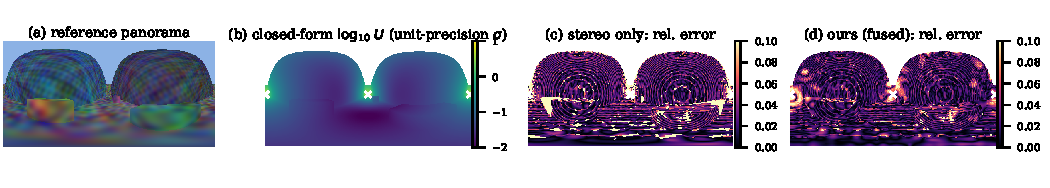
\includegraphics[width=\linewidth]{figures/teaser.pdf}
  \caption{\textbf{Two panoramas see depth only away from the epipoles.} (a) Reference panorama of a
  procedural street; the second panorama was taken 4\,m further down the road. (b) Our closed-form
  triangulation uncertainty at unit matching precision. It blows up at the two epipoles
  (\textcolor{gray}{$\times$}), which look along the street, exactly where the road continues.
  (c) Stereo alone fails in those regions. (d) Weighting stereo by the calibrated uncertainty and
  fusing it with a monocular prior keeps the stereo accuracy where it exists and falls back to the
  prior where it does not.}
  \label{fig:teaser}
\end{figure*}

Street-level panoramas cover most cities many times over. If one or two of them could be turned into
metric 3D geometry close to LiDAR quality, dense city models would become much cheaper to build and to
keep current. Two lines of work come close. Panoramic depth foundation
models~\cite{lin2026dap,da360,pager2026,rey2022360monodepth} predict depth for every direction from a
single image, but even the strongest report relative errors of several percent; at 20\,m that is more
than a metre. Generalizable multi-view methods for
panoramas~\cite{chen2023panogrf,chen2025splatter360,zhang2024pansplat} build spherical cost volumes
from two or more images, but they are trained to synthesize new views, not to produce calibrated metric
geometry.

Two high-resolution panoramas a few metres apart contain far more metric information than either line
of work uses explicitly. That information is spread very unevenly over the sphere, though.
Triangulation error grows with the square of the depth, and it diverges at the \emph{epipoles}, the two
directions along the baseline. A camera on a car or a backpack moves along the street, so the baseline
points down the street, and the region with no parallax is precisely the road ahead and behind
(\cref{fig:teaser}b). A depth estimator that ignores this has two bad options: distrust stereo
everywhere, or trust it in places where it means nothing.

This paper makes that structure explicit and builds the fusion around it. Concretely, we contribute:
\begin{itemize}
  \item A \textbf{closed-form uncertainty} for spherical two-view triangulation, for every ray, that
  also accounts for rotation and translation errors of the relative pose (\cref{sec:sigma}). It agrees
  with Monte Carlo simulation to within 0.5\%.
  \item A \textbf{calibration conditioned on that geometry} (\cref{sec:calibration}). Depth, baseline,
  epipoles, resolution and pose error all stay in the closed form; only the photometric matching
  precision is learned, as a two-parameter monotone map fitted robustly on teacher data.
  \item \textbf{Epipole-aware Bayesian fusion} of a learned panoramic prior with one or more stereo
  partners in log-depth (\cref{sec:fusion}). It corrects the prior's metric scale and rejects
  occlusions and moving objects with a mixture model. It returns metric depth with a per-ray
  uncertainty, and with a single panorama it reduces to the prior.
  \item A \textbf{city-as-teacher} scheme (\cref{sec:teacher}). A dense capture of one city supplies
  triangulation covariances for weighting the supervision, amodal targets behind occluders that only
  other panoramas see, and calibration data. So far we have tested only the last of these uses.
  \item A \textbf{controlled study} against geometry-blind baselines fitted on the same data
  (\cref{sec:experiments}). Without pose error, a well-calibrated match confidence does as well as the
  closed form. With pose error, or with an exposure-robust matching cost, it does not.
\end{itemize}
All experiments use procedural street scenes with exact ground truth. There are \emph{no real-data
experiments} in this draft. \Cref{sec:limitations} describes the KITTI-360~\cite{liao2022kitti360}
protocol with accumulated LiDAR that we consider the most important missing piece.

\section{Related Work}
\label{sec:related}

\paragraph{Monocular panoramic depth.}
Early 360$^\circ$ depth networks fuse equirectangular and cubemap features
\cite{wang2020bifuse,jiang2021unifuse,li2022omnifusion}, or merge perspective tangent-image
predictions \cite{rey2022360monodepth}. Recent foundation models predict metric depth for indoor
and outdoor panoramas \cite{lin2026dap,da360} or lift perspective foundation models such as Depth
Anything~\cite{yang2024depthv2} to the sphere \cite{pager2026}. Perspective metric-depth models
\cite{yin2023metric3d,piccinelli2024unidepth,bochkovskii2025depthpro} share the same limitation: a
single image constrains metric scale only through learned priors. We treat any such model as a
prior with a self-reported uncertainty and correct its scale with geometry.

\paragraph{Multi-view panoramic reconstruction.}
Omnidirectional stereo with spherical sweeps dates back to OmniMVS~\cite{won2019omnimvs}.
Generalizable radiance-field and Gaussian-splatting methods for wide-baseline panoramas
\cite{chen2023panogrf,chen2025splatter360,zhang2024pansplat} build spherical cost volumes and are
trained for view synthesis. Pointmap regressors \cite{wang2024dust3r,leroy2024mast3r,wang2025vggt}
reconstruct from unposed perspective images. None of these models the per-direction observability
of the two-view geometry explicitly or outputs calibrated metric uncertainty.

\paragraph{Triangulation uncertainty.}
First-order error propagation for triangulation is classical
\cite{hartley2003multiple,forstner2016photogrammetric}, and multi-view stereo pipelines
\cite{schoenberger2016mvs} use triangulation angles as heuristics for view selection. We derive
the closed form for spherical cameras including relative-pose error, use it as the scale-free
backbone of a calibrated uncertainty, and fuse with it rather than threshold it.

\paragraph{Uncertainty in depth estimation.}
Learned aleatoric uncertainty~\cite{kendall2017uncertainties}, self-supervised depth
uncertainty~\cite{poggi2020uncertainty} and sparsification metrics~\cite{ilg2018uncertainty}
evaluate how well predicted uncertainty ranks errors; calibrated regression~\cite{kuleshov2018calibrated}
recalibrates it post hoc. Our calibration is conditioned on a closed-form geometric quantity that
also carries relative-pose error, which a learned confidence cannot observe (\cref{sec:pose}).

\paragraph{Teacher supervision from more views.}
Behind the Scenes~\cite{wimbauer2023bts} and its distilled variant~\cite{han2024kdbts} train
single-view density fields using additional views as supervision on KITTI-360. Our teacher is a
metric multi-view reconstruction of a whole city whose per-point covariance weights the loss, and
which also supplies amodal targets and the calibration data.

\section{Method}
\label{sec:method}

\paragraph{Setting.}
We want the depth of a reference equirectangular panorama $I_1$ of width $W$. We are given a monocular
depth prior and, optionally, one or more partner panoramas $I_k$. Their relative poses
$(\mathbf{R}_k,\bvec_k)$ are expressed in the reference camera frame and come from GNSS/IMU or from
structure from motion~\cite{schoenberger2016sfm}. Each pixel defines a unit ray $\dvec$, and for each
ray we estimate the metric depth $z$, measured as distance along $\dvec$, together with its
uncertainty. All fusion is done in log-depth $\ell=\log z$, where relative errors add.

\subsection{Closed-form spherical triangulation uncertainty}
\label{sec:sigma}

% Two-view spherical triangulation geometry (TikZ).
\begin{figure}[t]
  \centering
  \begin{tikzpicture}[scale=0.95, >=Stealth, font=\footnotesize]
    % epipolar cones (unobservable depth) along the baseline line
    \fill[red!12] (0,0) -- (-1.6,0.42) arc[start angle=165, end angle=195, radius=1.65] -- cycle;
    \fill[red!12] (4,0) -- (5.6,0.42) arc[start angle=15, end angle=-15, radius=1.65] -- cycle;
    \node[red!70!black, align=center] at (-1.25,-0.75) {epipolar cone\\(no parallax)};
    % baseline
    \draw[thick] (0,0) -- node[below] {$\mathbf{b}$} (4,0);
    \draw[dashed, gray] (-1.7,0) -- (0,0); \draw[dashed, gray] (4,0) -- (5.7,0);
    % cameras (spheres)
    \draw[fill=blue!8] (0,0) circle (0.28); \node at (0,-0.55) {$\mathbf{C}_1$};
    \draw[fill=orange!12] (4,0) circle (0.28); \node at (4,-0.55) {$\mathbf{C}_2$};
    % point and rays
    \coordinate (X) at (1.3,2.6);
    \fill (X) circle (1.4pt); \node[anchor=east] at ($(X)+(-0.35,0.15)$) {$\mathbf{X}=z\,\mathbf{d}$};
    \draw[->, blue!70!black, thick] (0,0) -- (X);
    \draw[->, orange!80!black, thick] (4,0) -- (X);
    % angles
    \draw (0.5,0) arc[start angle=0, end angle=63.4, radius=0.5]; \node at (0.68,0.36) {$\alpha$};
    \draw (3.45,0) arc[start angle=180, end angle=116.2, radius=0.55]; \node at (3.28,0.38) {$\beta$};
    \draw ($(X)+(-0.17,-0.33)$) arc[start angle=243.4, end angle=296.2, radius=0.37]; \node at (1.36,1.95) {$\gamma$};
    % uncertainty ellipse along ray 1
    \draw[blue!60, fill=blue!10, rotate around={63.4:(X)}] (X) ellipse (0.45 and 0.09);
    \node[blue!60!black, anchor=west] at (2.15,2.55) {$\sigma_z \propto \dfrac{z^2}{\|\mathbf{b}\|\sin\alpha}$};
  \end{tikzpicture}
  \caption{\textbf{Spherical two-view geometry.} The depth $z$ along the reference ray $\mathbf{d}$
  follows from the law of sines; its uncertainty (\cref{eq:sigma}) grows quadratically with depth and
  diverges inside the epipolar cones along the baseline, which for street-level capture is the
  direction of travel.}
  \label{fig:geometry}
\end{figure}


Take one partner at $\bvec$ and a scene point $\mathbf{X}=z\dvec$. In the triangle
$(\mathbf{0},\bvec,\mathbf{X})$, let $\alpha$ be the angle at the reference camera between $\dvec$ and
$\bvec$, let $\beta$ be the angle at the partner, and let $\gamma=\pi-\alpha-\beta$ be the parallax
angle at $\mathbf{X}$ (\cref{fig:geometry}). By the law of sines,
\begin{equation}
  z = \|\bvec\|\,\frac{\sin\beta}{\sin\gamma}.
\end{equation}
Matching noise tilts the two observed directions by small angles. Only the components inside the
epipolar plane change $z$ to first order, and differentiating gives
$\partial z/\partial\alpha=\|\bvec\|\sin\beta\cos\gamma/\sin^2\gamma$ and
$\partial z/\partial\beta=\|\bvec\|\sin\alpha/\sin^2\gamma$. Pose errors enter in two ways. A rotation
error of the partner, with per-axis standard deviation $\sigma_R$, turns its ray inside the epipolar
plane by the same angle. A position error, with per-axis standard deviation $\sigma_t$, shifts the
partner ray sideways. Only the in-plane component perpendicular to the ray matters, and it moves the
intersection by $\delta/\sin\gamma$. With angular matching precision $\sigma_\theta$ on both rays,
\begin{equation}
  \sigma_z^2 = \frac{\|\bvec\|^2}{\sin^4\gamma}\Big[\sigma_\theta^2\sin^2\beta\cos^2\gamma
  + (\sigma_\theta^2+\sigma_R^2)\sin^2\alpha\Big] + \frac{\sigma_t^2}{\sin^2\gamma}.
  \label{eq:sigma}
\end{equation}
Far from the cameras ($z\gg\|\bvec\|$, so $\beta\to\pi-\alpha$) and without pose error, this simplifies
to $\sigma_z\approx\sqrt{2}\,\sigma_\theta z^2/(\|\bvec\|\sin\alpha)$. The error grows with the square
of the depth, shrinks with a longer baseline, and diverges at the epipoles $\alpha\in\{0,\pi\}$.

One implementation detail matters in practice. For distant points the parallax angle is tiny, and
computing $\sin\gamma$ as $\sqrt{1-\cos^2\gamma}$ in single precision loses essentially all
significant digits. We compute every sine from a cross-product norm instead. To check the derivation,
we triangulated with isotropic angular noise on both rays and random pose perturbations in a Monte
Carlo simulation. \Cref{eq:sigma} matched the simulated spread to within 0.5\% in every
configuration we tried (the checks are part of the released unit tests).

We write $\U(\dvec)=\sigma_z/z$ for the log-depth uncertainty at \emph{unit} matching precision, one
pixel or $\sigma_\theta=2\pi/W$, without pose error, and $P(\dvec)$ for the pose-only term. $\U$
contains all of the geometry: depth, baseline length and direction, and image resolution. It depends
on the unknown depth, so we evaluate it at the scale-aligned prior depth. The stereo estimate would be
the wrong choice: it is least reliable exactly where $\U$ is large.

\subsection{Spherical plane-sweep stereo}
\label{sec:stereo}

For every reference ray and every log-depth hypothesis, we project $z\dvec$ into the partner panorama
and sample it, wrapping around in longitude. A coarse pass sweeps 64 log-spaced hypotheses between 1
and 200\,m. Two refinement passes of 16 hypotheses each follow around the best match, and we take the
soft-arg-min of the last pass. As matching cost we use either the box-aggregated L1 difference or
$1-$ZNCC over a $5\times5$ window; the latter is unaffected by gain and bias changes between captures.
The match confidence is the distinctiveness of the coarse cost curve,
$c=(\operatorname{med}_h C_h-\min_h C_h)/\operatorname{med}_h C_h$. It drops to zero near the epipoles,
where every hypothesis lands on almost the same pixel, and in textureless or occluded regions.

\subsection{Geometry-conditioned calibration}
\label{sec:calibration}

\Cref{eq:sigma} is exact \emph{for a given} $\sigma_\theta$. The catch is that the effective matching
precision is not a fixed number of pixels. It depends on the aggregation window, the texture, the cost
function and the bounded depth search. On our benchmark, the implied precision ranges from about
$0.1$\,px near the epipoles to $0.6$\,px perpendicular to the baseline. We therefore keep the geometry
in closed form and learn only a monotone map from $\U$ to the observed error:
\begin{equation}
  \sigma_s(\dvec) = \sqrt{\big(a(c)\,\U(\dvec)^{\kappa}\big)^2 + P(\dvec)^2},
  \label{eq:calibration}
\end{equation}
where the exponent $\kappa$ is shared and the scale $a(c)$ is piecewise constant and non-increasing in
the match confidence $c$ (six quantile bins). The pose term $P$ has no free parameters. We fit the
parameters on calibration rays with known depth, which in practice come from the city teacher of
\cref{sec:teacher}. The exponent $\kappa$ is chosen by maximizing a Student-$t$ likelihood ($\nu=3$),
which tolerates occlusions and mismatches. Each scale $a$ is then fitted by Gaussian maximum likelihood
on the $t$-inliers. The second step is needed because fusion requires a standard deviation, and the
$t$-scale underestimates it by roughly 20\% when errors are Gaussian. Rays deep inside the epipolar
cones are left out of the fit, since the bounded depth range truncates their errors. Setting $\kappa=1$
with a single bin recovers the pure closed form with a constant $\sigma_\theta$.

\subsection{Epipole-aware fusion}
\label{sec:fusion}

\paragraph{Scale alignment.}
Monocular metric depth is frequently off by a per-image scale factor. We estimate a global log-scale
offset $\hat o$ as the precision-weighted median of $\mu_s-\mu_p$ over well-conditioned rays
($\sigma_s<0.05$, $c>0.5$), with weights $c/\sigma_s^2$. Its robust standard error is
$s_o=1.2533\cdot1.4826\,\mathrm{MAD}/\sqrt{n/25}$. The ray count $n$ is divided by 25 because errors
are correlated within each $5\times5$ aggregation window. We place a Gaussian prior
$\mathcal{N}(0,s_p^2)$ on the scale error of the depth prior, with $s_p=0.1$, and apply the posterior
mean $o=\hat o\,s_p^2/(s_p^2+s_o^2)$. When only a few reliable rays remain, or they disagree with each
other, as happens under strong photometric degradation, the correction shrinks towards zero rather
than locking onto a wrong scale.

\paragraph{Gated Bayesian fusion.}
In log-depth, the prior is $\mathcal{N}(\mu_p,\sigma_p^2)$ and partner $k$ contributes
$\mathcal{N}(\mu_k,\sigma_k^2)$ with confidence $c_k$. Occlusions, moving objects and mismatches cause
gross errors. We therefore model the disagreement $\delta_k=\mu_k-\mu_p$ as a mixture of an inlier
Gaussian $\mathcal{N}(0,\sigma_p^2+\sigma_k^2)$, with prior probability $\pi$, and a uniform outlier
over the log-depth range $L$:
\begin{equation}
  w_k = c_k\,\frac{\pi\,\mathcal{N}(\delta_k;0,\sigma_p^2+\sigma_k^2)}
  {\pi\,\mathcal{N}(\delta_k;0,\sigma_p^2+\sigma_k^2)+(1-\pi)/L}.
\end{equation}
The fused estimate is then
\begin{equation}
  \frac{1}{\sigma^2}=\frac{1}{\sigma_p^2}+\sum_k\frac{w_k}{\sigma_k^2},\qquad
  \mu=\sigma^2\Big(\frac{\mu_p}{\sigma_p^2}+\sum_k\frac{w_k\,\mu_k}{\sigma_k^2}\Big).
\end{equation}
Near the epipoles $\sigma_k\to\infty$, and the result is simply the scale-aligned prior. Perpendicular
to the baseline, stereo dominates. With a single panorama there are no partners, and the output is the
prior. Every step is differentiable, so the module can also sit inside a learned network
(\cref{sec:teacher}).

\subsection{City as teacher}
\label{sec:teacher}

Suppose one city has been captured densely, with many panoramas per street. We reconstruct it once with
multi-view geometry, using SfM and MVS~\cite{schoenberger2016sfm,schoenberger2016mvs} or surface
splatting~\cite{huang2024twodgs}. A teacher point $\mathbf{X}$ seen from centres $\mathbf{C}_i$ at
distances $r_i$, along unit directions $\mathbf{u}_i$, has triangulation information
$\boldsymbol{\Lambda}=\sum_i(\mathbf{I}-\mathbf{u}_i\mathbf{u}_i^\top)/(r_i\sigma_\theta)^2$ and
covariance $\boldsymbol{\Sigma}=\boldsymbol{\Lambda}^{-1}$. We invert in double precision, because
points seen from a single view give nearly singular matrices. For a student panorama we render targets
in two layers. The first is the nearest teacher surface along each ray. The second is the first surface
behind it, for example behind a parked car or around a corner, which only other panoramas of the city
observe. Each target carries its variance $\dvec^\top\boldsymbol{\Sigma}\dvec$ along the student ray.
A student that predicts $(\mu,\sigma)$ in log-depth is trained with a Gaussian negative log-likelihood
of variance $\sigma^2+\dvec^\top\boldsymbol{\Sigma}\dvec/z^2$. Poorly triangulated teacher points
therefore supervise weakly instead of wrongly. The same teacher also provides the calibration rays for
\cref{eq:calibration}. Our reference student uses one equirectangular encoder, with wrap-around padding
in longitude, that feeds five components: a prior head, a stereo cost volume on learned features, the
closed-form uncertainty with a learned global scale, the fusion above, and an amodal second-layer head.

\section{Experiments}
\label{sec:experiments}

\subsection{Setup}

\paragraph{Benchmark.}
Real street panoramas with dense metric ground truth are not available to us at the time of writing
(\cref{sec:limitations}). We therefore use procedural street canyons with exact depth: a ground plane,
two building fa\c{c}ades 5--9\,m from the camera with random heights, end walls 60--120\,m away,
3--7 box-shaped parked vehicles, and sky. All surfaces carry a view-independent multi-scale procedural
texture. The reference panorama is at the origin and the partner $b$ metres further along the street,
the hardest configuration, because the epipoles look down the street. Unless stated otherwise,
panoramas are $256\times512$ and $b=4$\,m. The monocular prior is simulated as the true log-depth plus
spatially smooth noise with 6\% standard deviation and a global scale error drawn uniformly in
$\pm10\%$, with a constant self-reported $\sigma_p=0.06$; this matches the reported accuracy of current
panoramic foundation models~\cite{lin2026dap}. Calibration uses six scenes (seeds $\geq1000$), disjoint
from the ten test scenes, with ground truth standing in for the city teacher.

\paragraph{Baselines.}
All fusion variants share the same stereo, prior, scale alignment and gate, and differ only in the
stereo uncertainty $\sigma_s$:
\emph{constant} ($\sigma_s=s$) and \emph{confidence} ($\sigma_s=s/c$), with $s$ fitted on the same
calibration rays and with the same robust estimator as ours; \emph{selection}, which takes per ray the
source with the smaller calibrated $\sigma$; and our closed form without calibration
($\sigma_\theta=0.5$\,px). We also report the prior alone, the scale-aligned prior and stereo alone.

\paragraph{Metrics.}
Median relative depth error overall and per bin of the angle between ray and baseline; the fraction
of rays within 20\,cm; the fraction of errors within the predicted $1\sigma$ (ideal 0.683); the Gaussian
negative log-likelihood (NLL) in log-depth, a proper scoring rule for the predicted distribution;
and the area under the sparsification error curve (AUSE)~\cite{ilg2018uncertainty}.

\subsection{Main results}

\begin{table*}[t]
  \centering
  \resizebox{\linewidth}{!}{\begin{tabular}{l ccccc c ccc}
\toprule
 & \multicolumn{5}{c}{Median rel.\ error (\%) $\downarrow$, by angle to baseline} & $<$20\,cm (\%) $\uparrow$ & Cal.\ $1\sigma$ & NLL $\downarrow$ & AUSE $\downarrow$ \\
\cmidrule(lr){2-6}
Method & 0--10$^\circ$ & 10--30$^\circ$ & 30--60$^\circ$ & 60--90$^\circ$ & all & all & (0.68) & all & all \\
\midrule
Prior only & 6.81 & 7.04 & 6.99 & 6.92 & 6.95 & 29.80 & 0.44 & -0.73 & 0.481 \\
Prior + scale alignment & 4.45 & 4.03 & 3.83 & 3.98 & 3.94 & 47.12 & 0.69 & -1.40 & 0.534 \\
Stereo only & 21.07 & 3.03 & 2.05 & 1.49 & 1.78 & 68.99 & \textbf{0.68} & 26.04 & 0.386 \\
\midrule
Fusion, constant $\sigma_s$ & 4.90 & 2.41 & 1.76 & 1.48 & 1.64 & 73.66 & 0.73 & -2.17 & \textbf{0.329} \\
Fusion, confidence $\sigma_s$ & 4.49 & \textbf{2.35} & \textbf{1.73} & 1.43 & \textbf{1.60} & \textbf{74.10} & 0.73 & \textbf{-2.22} & 0.331 \\
Selection (min.\ $\sigma$) & 4.45 & 3.07 & 2.03 & 1.47 & 1.74 & 70.60 & 0.70 & -2.03 & 0.354 \\
Ours, closed form ($\sigma_{px}{=}0.5$) & 4.38 & 3.03 & 1.91 & 1.43 & 1.67 & 72.17 & 0.63 & -1.36 & 0.461 \\
Ours (calibrated) & \textbf{4.30} & 2.63 & 1.77 & \textbf{1.41} & 1.61 & 73.63 & 0.71 & -2.16 & 0.361 \\
\bottomrule
\end{tabular}}
  \caption{\textbf{Main results} ($256\times512$, $b=4$\,m along the street, 10 test scenes). The
  calibrated closed form is best or tied in accuracy near the epipoles and orthogonal to the baseline,
  and is well calibrated. A geometry-blind confidence-based $\sigma_s$, fitted on the same calibration
  data, is equally accurate in this in-distribution setting (see text).}
  \label{tab:main}
\end{table*}

\begin{figure}[t]
  \centering
  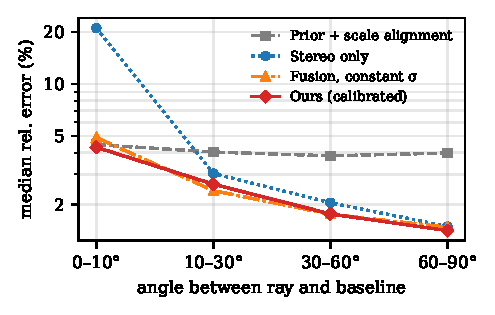
\includegraphics[width=\linewidth]{figures/error_vs_angle.pdf}
  \caption{Median relative error versus the angle between ray and baseline. Stereo diverges near the
  epipoles; the scale-aligned prior is flat; fusion follows the lower envelope.}
  \label{fig:angle}
\end{figure}

\Cref{tab:main,fig:angle} show the expected structure. Stereo alone is accurate orthogonal to the
baseline (1.49\% at 60--90$^\circ$) but useless near the epipoles (21\%). The prior is uniformly
mediocre, 6.95\% before and 3.94\% after scale alignment. Our fusion follows the lower envelope of the
two, reducing the median error of the raw prior from 6.95\% to 1.61\% overall while remaining
calibrated (0.71 of errors within $1\sigma$). Scale alignment matters: without it the error near the
epipoles rises from 4.30\% to 6.51\%. Evaluating $\U$ at the stereo depth is equivalent once the
precision is calibrated. The uncalibrated closed form ($\sigma_\theta=0.5$\,px) is as accurate overall
but badly calibrated (NLL $-1.36$ vs.\ $-2.16$), which motivates \cref{eq:calibration}: on this
benchmark, the implied matching precision varies by $6\times$ with the angle to the baseline.

\paragraph{An honest negative result.}
With its scale fitted on the same calibration rays, the geometry-blind \emph{confidence} baseline is as
accurate as ours in-distribution (1.60\% vs.\ 1.61\%) and has a slightly better NLL. The match
confidence already collapses near the epipoles, because all hypotheses project to nearly the same
pixel, so it implicitly encodes much of the observability. The same holds when transferring the
calibration to other baselines and resolutions (\cref{tab:transfer}): all calibrated fusion variants
are within 0.1 percentage points of each other. The closed form therefore does \emph{not}
improve accuracy over a well-calibrated confidence in the absence of pose error on this benchmark.

\begin{table*}[t]
  \centering
  \small
  \begin{tabular}{l cccccccc}
\toprule
 & \multicolumn{2}{c}{$b{=}2$\,m} & \multicolumn{2}{c}{$b{=}8$\,m} & \multicolumn{2}{c}{128$\times$256} & \multicolumn{2}{c}{512$\times$1024} \\
\cmidrule(lr){2-3}\cmidrule(lr){4-5}\cmidrule(lr){6-7}\cmidrule(lr){8-9}
Method & Med.\,(\%) & NLL & Med.\,(\%) & NLL & Med.\,(\%) & NLL & Med.\,(\%) & NLL \\
\midrule
Prior + scale alignment & 3.92 & -1.39 & 3.91 & -1.39 & 3.99 & -1.37 & 3.97 & -1.39 \\
Stereo only & 1.65 & 2.02 & 2.16 & 133.00 & 2.21 & 5.59 & 1.49 & 75.30 \\
Fusion, constant $\sigma_s$ & 1.57 & -2.25 & 1.82 & -1.87 & 1.94 & -2.03 & 1.46 & -2.18 \\
Fusion, confidence $\sigma_s$ & 1.52 & -2.32 & 1.81 & -1.92 & 1.89 & -2.10 & 1.41 & -2.22 \\
Ours (calibrated) & 1.51 & -2.29 & 1.82 & -1.89 & 1.97 & -2.03 & 1.38 & -2.00 \\
\bottomrule
\end{tabular}
  \caption{\textbf{Transfer without recalibration}: all methods are calibrated at $b=4$\,m and
  $256\times512$, and evaluated at other baselines and resolutions (5 scenes; 3 at $512\times1024$).}
  \label{tab:transfer}
  \label{sec:transfer}
\end{table*}

\subsection{Where geometry matters: relative-pose error}
\label{sec:pose}

\begin{table*}[t]
  \centering
  \small
  \begin{tabular}{l ccccccccc}
\toprule
 & \multicolumn{3}{c}{0.1$^\circ$/2cm} & \multicolumn{3}{c}{0.3$^\circ$/5cm} & \multicolumn{3}{c}{1$^\circ$/10cm} \\
\cmidrule(lr){2-4}\cmidrule(lr){5-7}\cmidrule(lr){8-10}
Method & Med. & Cal. & NLL & Med. & Cal. & NLL & Med. & Cal. & NLL \\
\midrule
Constant $\sigma_s$ & 1.77 & 0.70 & -2.08 & 2.34 & 0.59 & -1.70 & 3.99 & 0.44 & -0.50 \\
Constant $\sigma_s$, refit & 1.79 & 0.73 & -2.09 & 2.41 & 0.71 & -1.83 & 6.77 & 0.44 & -0.77 \\
Confidence $\sigma_s$ & \textbf{1.73} & 0.70 & -2.13 & 2.30 & 0.60 & -1.79 & 3.93 & 0.46 & -0.68 \\
Confidence $\sigma_s$, refit & 1.74 & 0.72 & \textbf{-2.13} & 2.36 & 0.71 & -1.87 & 6.52 & 0.44 & -0.82 \\
Ours w/o pose term & 1.74 & \textbf{0.69} & -2.08 & \textbf{2.26} & 0.60 & -1.78 & 3.86 & 0.46 & -0.68 \\
Ours & 1.75 & 0.71 & -2.09 & 2.28 & \textbf{0.70} & \textbf{-1.89} & \textbf{3.39} & \textbf{0.67} & \textbf{-1.54} \\
\bottomrule
\end{tabular}
  \caption{\textbf{Relative-pose error.} The partner pose given to all methods is perturbed by
  rotation/translation noise with the stated per-axis standard deviations; images are rendered with the
  true poses. ``refit'': geometry-blind baselines recalibrated on calibration scenes with the same pose
  noise. Ours uses the known noise level in the closed-form pose term (\cref{eq:sigma}) and is
  \emph{not} recalibrated. 8 test scenes.}
  \label{tab:pose}
\end{table*}

Poses from GNSS/IMU or SfM are never exact, and their error affects rays very differently: by
\cref{eq:sigma}, a translation error moves the depth by $\delta/\sin\gamma$, which is negligible
for close points orthogonal to the baseline and dominant for distant points and near the epipoles. Match
confidence cannot see this, because the cost curve can be sharply peaked at a wrong depth.
\Cref{tab:pose} injects pose errors into the partner pose. For small errors ($0.1^\circ$, 2\,cm) all methods are
equivalent. At $0.3^\circ$/5\,cm the geometry-blind uncertainties become over-confident (0.59--0.60 of
errors within $1\sigma$), while ours stays calibrated (0.70) and has the best NLL, at equal accuracy.
At $1^\circ$/10\,cm the pose term changes the result: ours reduces the median error from 3.93\% (best
baseline) to 3.39\%, raises the in-$1\sigma$ fraction from 0.46 to 0.67, and improves the NLL from
$-0.82$ to $-1.54$. Refitting the geometry-blind baselines under the same pose noise restores
calibration at moderate noise. At large noise, however, it inflates $\sigma_s$ uniformly, so no ray
remains reliable enough for scale alignment and the result degrades towards the unaligned prior
(6.5--6.8\%). Ours keeps rays orthogonal to the baseline at close range trustworthy, because there the pose
term is small. The pose term assumes the noise level is known; in practice it would come from the
SfM covariance or the GNSS/IMU specification.

\paragraph{Partners with different baselines.}
With two partners at $+2$\,m and $-8$\,m, all calibrated variants reach the same accuracy
(1.19--1.21\%) and similar calibration, \ie we observe no benefit of geometric weighting across
partners on this benchmark.

\subsection{Capture effects}
\label{sec:capture}

\begin{table}[t]
  \centering
  \footnotesize
  \setlength{\tabcolsep}{1.8pt}
  \begin{tabular}{l ccccc}
\toprule
Method & clean & exposure & noise & moving cars & all \\
\midrule
Confidence $\sigma_s$, L1 & \textbf{1.59} & 5.69 & 2.26 & \textbf{1.62} & 9.07 \\
Confidence $\sigma_s$, ZNCC & 5.29 & 5.42 & 6.50 & 5.32 & 6.72 \\
Ours, L1 & 1.60 & 5.96 & \textbf{2.24} & 1.63 & 8.51 \\
Ours, ZNCC, w/o outlier gate & 3.06 & 3.06 & 3.95 & 3.09 & 4.57 \\
Ours, ZNCC & 2.80 & \textbf{2.88} & 3.92 & 2.82 & \textbf{4.56} \\
\bottomrule
\end{tabular}
  \caption{\textbf{Capture effects} (median relative error, \%, 8 scenes): partner exposure change
  (gain 0.6, bias 0.15), sensor noise ($\sigma=0.03$), half of the parked cars moved by 3\,m between
  captures, and all three combined. Each cost function has its own calibration.}
  \label{tab:capture}
\end{table}

\Cref{tab:capture} varies the capture conditions. Two findings stand out. First, the cost
function matters: L1 is best for clean images and under sensor noise, while ZNCC is far more robust to
an exposure change between captures (2.88\% vs.\ 5.96\%) and in the combined setting (4.56\%
vs.\ 8.51\%). Second, with ZNCC the geometry-blind confidence baseline breaks down (5.29\% vs.\ 2.80\%
on clean data, 6.72\% vs.\ 4.56\% combined). Its success with L1 rests on the L1 confidence happening
to encode the epipolar degeneracy, which does not hold for every cost. The closed form does not depend
on such a coincidence. The outlier gate gives a modest gain on clean data and with moving cars
(3.06\%$\to$2.80\% and 3.09\%$\to$2.82\%), and none in the combined setting.

\subsection{Calibrating from a noisy city teacher}
\label{sec:teacher_cal}

\begin{table}[t]
  \centering
  \footnotesize
  \setlength{\tabcolsep}{3pt}
  \begin{tabular}{l c ccc}
\toprule
Calibration data & $\kappa$ & Med.\ rel.\ (\%) & Cal.\ $1\sigma$ & NLL \\
\midrule
Ground truth (oracle) & 0.38 & 1.61 & 0.71 & -2.16 \\
\midrule
Teacher, naive & 0.40 & 1.62 & 0.73 & -2.15 \\
Teacher, $\geq$2 views & 0.35 & 1.62 & 0.73 & -2.16 \\
Teacher, covariance-aware (ours) & 0.30 & 1.61 & 0.73 & -2.17 \\
\bottomrule
\end{tabular}
  \caption{\textbf{Calibration data.} The precision model of \cref{eq:calibration} is fitted on depth
  from a simulated city teacher (7 panoramas per street, lateral offsets, points displaced by draws
  from their own triangulation covariance, 0.5\,px matching at 2048\,px width) instead of ground truth.
  Evaluation as in \cref{tab:main}.}
  \label{tab:teacher}
\end{table}

Fitting the calibration on noisy teacher depth instead of ground truth costs nothing
measurable (\cref{tab:teacher}): all variants reach 1.61--1.62\% with calibrated uncertainties. Treating
the teacher as exact inflates the fitted scales slightly, as expected, because teacher error is
absorbed into the matching precision. Adding the teacher covariance in quadrature removes this
inflation. Downstream, however, the difference is negligible here, because the simulated teacher is
about $8\times$ more precise than the $512$\,px stereo it calibrates. Covariance-aware calibration
should matter only for teachers of comparable precision; we have not tested that regime.

\section{Limitations and Future Work}
\label{sec:limitations}

\paragraph{No real data yet.}
Every result in this draft comes from procedural scenes with a simulated prior. Real panoramas bring
non-Lambertian surfaces, vegetation, sky, rolling-shutter and stitching artefacts, and a prior whose
errors have spatial structure that our simulation does not reproduce. The experiment that will decide
the matter is KITTI-360~\cite{liao2022kitti360}. Its two 180$^\circ$ fisheye cameras (MEI
model~\cite{mei2007single}) cover nearly the full sphere and can be resampled to equirectangular
images, and its accumulated LiDAR provides metric ground truth, including in occluded regions. We plan
to use pairs of frames 2--8\,m apart along the trajectory, priors from Depth Any
Panoramas~\cite{lin2026dap} and DA360~\cite{da360}, calibration on training sequences, and evaluation
on held-out sequences. The comparison will include Splatter-360~\cite{chen2025splatter360},
PanSplat~\cite{zhang2024pansplat}, and pointmap regressors~\cite{leroy2024mast3r,wang2025vggt} run on
cube faces.

\paragraph{The learned student is untested.}
The city-as-teacher training of \cref{sec:teacher} is implemented. A small reference student trained
for 400 steps on a CPU did not converge, and its errors stayed far above those of the prior, so we
report no student results. The teacher has been tested only as a source of calibration data
(\cref{sec:teacher_cal}). Whether amodal supervision and covariance-weighted teacher losses help a
foundation-model student will require training on GPUs.

\paragraph{Modelling assumptions.}
Partners share the reference image, so treating several of them as independent overstates the
precision. Moving objects are rejected as outliers, and in those regions the depth comes from the
prior. Relative-pose error enters $\sigma_s$ only through a per-axis standard deviation. When poses
come from SfM, the full pose covariance should be propagated instead.

\section{Conclusion}
Two panoramas hold precise metric information about a scene, but only away from their epipoles. A
closed-form, pose-aware triangulation uncertainty, with a small calibration of the matching precision,
makes this explicit. Fused on that basis with a monocular prior, it yields metric depth with a per-ray
uncertainty, and falls back to the prior where the geometry says nothing. In our controlled
experiments it cuts the error of a simulated foundation prior by more than $4\times$. Without pose
error, a well-calibrated match confidence does just as well. The closed form is clearly better once
the relative pose is uncertain, which is the usual situation for street-level capture, and when an
exposure-robust cost is used, because the match confidence then no longer encodes the epipoles.
Whether all this brings real street-level panoramas close to LiDAR accuracy is the next question to
answer.

{
    \small
    \bibliographystyle{ieeenat_fullname}
    \bibliography{main}
}
\end{document}
